\documentclass[english]{acm_proc_article-sp}
%\documentclass[a4paper,ngerman,english]{amsbook} % Use book format.
\usepackage[T1]{fontenc}
\usepackage[utf8]{inputenc}
\usepackage{verbatim}
\usepackage{hyperref}
\usepackage{graphicx}
\usepackage{pifont}

\usepackage{enumerate}

\newcommand{\tick}{\ding{51}}
\newcommand{\fattick}{\ding{51}}

\frenchspacing


% ============================================================
% Markup macros for proof-reading
\usepackage{ifthen}
\usepackage[normalem]{ulem} % for \sout
\usepackage{xcolor}
\newcommand{\ra}{$\rightarrow$}
\newboolean{showedits}
\setboolean{showedits}{true} % toggle to show or hide edits
\ifthenelse{\boolean{showedits}}
{
	\newcommand{\ugh}[1]{\textcolor{red}{\uwave{#1}}} % please rephrase
	\newcommand{\ins}[1]{\textcolor{blue}{\uline{#1}}} % please insert
	\newcommand{\del}[1]{\textcolor{red}{\sout{#1}}} % please delete
	\newcommand{\chg}[2]{\textcolor{red}{\sout{#1}}{\ra}\textcolor{blue}{\uline{#2}}} % please change
}{
	\newcommand{\ugh}[1]{#1} % please rephrase
	\newcommand{\ins}[1]{#1} % please insert
	\newcommand{\del}[1]{} % please delete
	\newcommand{\chg}[2]{#2}
}
% ============================================================
% Put edit comments in a really ugly standout display
%\usepackage{ifthen}
\newboolean{showcomments}
\setboolean{showcomments}{false}
\newcommand{\id}[1]{$-$Id: scg-llncs.tex 30911 2010-02-05 10:21:47Z oscar $-$}
\newcommand{\yellowbox}[1]{\fcolorbox{gray}{yellow}{\bfseries\sffamily\scriptsize#1}}
\newcommand{\triangles}[1]{{\sf\small$\blacktriangleright$\textit{#1}$\blacktriangleleft$}}
\ifthenelse{\boolean{showcomments}}
{\newcommand{\nbc}[3]{
 {\colorbox{#3}{\bfseries\sffamily\scriptsize\textcolor{white}{#1}}}
 {\textcolor{#3}{\sf\small$\blacktriangleright$\textit{#2}$\blacktriangleleft$}}}
 \newcommand{\version}{\emph{\scriptsize\id}}}
{\newcommand{\nbc}[3]{\textcolor{#3}{#2}}
 \newcommand{\version}{}}
\newcommand{\nb}[2]{\nbc{#1}{#2}{orange}}
\newcommand{\here}{\yellowbox{$\Rightarrow$ CONTINUE HERE $\Leftarrow$}}
\newcommand\rev[2]{\nb{TODO (rev #1)}{#2}} % reviewer comments
\newcommand\fix[1]{\nb{FIX}{#1}}
\newcommand\todo[1]{\nb{TO DO}{#1}}
\newcommand\meta[1]{\nbc{META}{#1}{purple}}
\newcommand\jr[1]{\nbc{JR}{#1}{orange}}
\newcommand\nes[1]{\nbc{nes}{#1}{blue}}
\newcommand\on[1]{\nbc{ON}{#1}{teal}} % add more author macros here
\newcommand\ewe[1]{\nbc{EWE}{#1}{olive}} % add more author macros here



\begin{document}
\conferenceinfo{WOODSTOCK}{'97 El Paso, Texas USA}
%\CopyrightYear{2007} % Allows default copyright year (20XX) to be over-ridden - IF NEED BE.
%\crdata{0-12345-67-8/90/01}  % Allows default copyright data (0-89791-88-6/97/05) to be over-ridden - IF NEED BE.
% --- End of Author Metadata ---

\title{DoodleDebug}

\numberofauthors{3}

\author{
\alignauthor Niko Schwarz \\
\affaddr{University of Bern}
\alignauthor Cedric Reichenbach \\
\affaddr{University of Bern}
\alignauthor Oscar Nierstrasz \\
\affaddr{University of Bern}
}

\date{1 March 2012}

\maketitle

\begin{abstract}
Software developers actively make use of debugging tools in order to find problem sources in code. In relation to a previous paper\cite{Schw11b}, we designed and implemented a tool representing a new style of debugging: Objects are responsible of their own visual representation, as already seen in classical tools, but with a powerful and yet simple mechanism for graphical visualization rather than text only. Most of its power is gained when taking on conceptually multidimensional objects like lists of matrices.
\end{abstract}


\section{Introduction}
Java's \verb-System.out.println()- 
allows developers to easily compare many temporal states of an object or many different instances beside each other, which may be a reason for its popularity;\nes{On one of the first pages of "programming pearls", the author notes that often it's easier to write "just writing println is often easier". That would fit here.} \meta{Do you mean p. 24, the customized letter?} \nes{I left my copy in Switzerland :(.} but when it comes to complex problems, like a list of matrices, \verb-System.out.println()- breaks down and becomes either expensive to use or completely useless\cite{Schw11b}.
Debuggers and object inspectors fare much better at showing the inners of objects, but unlike the console output of \verb-System.out.println()-, debugger and object inspectors only show one moment in time. There are a few notable exceptions to the previous sentence, to which we will come back. 

We believe that the popularity of \verb-System.out.println()- is in no small parts due to its simplicity in API and concept. DoodleDebug therefore aims to offer an API which is no more difficult than that of \verb-System.out.println()-. At the same time, we try to add it the advantages of two-dimensional layout, and a semantic zoom on objects that allows inspecting all instance variables recursively.

In a small qualitative study with 7 Java developers, we examine DoodleDebug's debugging performance compared to classical tools under the same conditions. We pose three different problems to each candidate to be alternately solved with or without DoodleDebug, recording with screen capture videos and think aloud protocol. Then we search for problematic situations experienced with one tool and see if they've been solved easier using other tools.

\section{DoodleDebug in a nutshell}
Developers can choose how objects of a class are to be doodled on a virtual canvas. When first doodling an object on the canvas, the doodle  will appear in the upper left corner, because the cursor is initially placed in the upper left corner. Doodling on the canvas advances the cursor to the right of the previous doodle. As seen in Figure~\ref{canvas-illustration}, the cursor can also be moved to the next line, or the next column. \nes{Compare this with println in related work.}

\begin{figure}[h]
	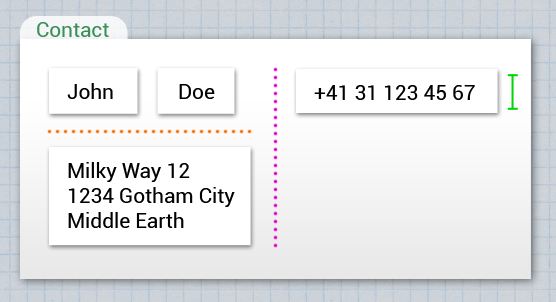
\includegraphics[width=\linewidth]{img/doodleable-example.png}
	\caption[Usage of the Doodleable interface]{Example of a \texttt{Contact} class' \texttt{doodleOn()} method. Dotted lines visualize the effect of the structuring methods \texttt{newLine()} (orange) and \texttt{newColumn()} (purple). The green i-beam indicates the final position of the canvas' imaginary cursor.}
	\meta{Can I make this wider? It's hard to read...}
	\label{canvas-illustration}
\end{figure}

As a more complex example, an entire address book is doodled by the developer as follows.
\begin{verbatim}
public class AddressBook implements Doodleable {
    ...

    public void doodleOn(DoodleCanvas c) {
        for (Contact contact : contacts) {
            c.draw(contact);
            c.newLine();
        }
    }

    public void summarizeOn(DoodleCanvas c) {
        c.draw("AddressBook with "
            + numberOfContacts() + " entries");
    }
}
\end{verbatim}
\meta{Should I add the code of \texttt{Contact} and \texttt{Address} as well? I'm afraid it'll grow too big with that...}
The resulting rendering is seen in Figure~\ref{addressbook_whole}.
Note that not all the state of the address book is visible in its doodle. However, all of it is available. Once the user clicks on any entry of the address book, an object inspector is opened, as seen in Figure~\ref{addressbook_contact}, that reveals a more detailed rendering of the clicked address. 

\nes{Add an example session of printing a non-trivial object across time.}

DoodleDebug allows to track the state of an object over a period of time by doodling it periodically. As an example, six players participate in a game with the goal to reduce other player's life point. Players with 0 points die, the last one standing wins.

\todo{include sceenshots and explain using them}

\begin{figure}[h]
	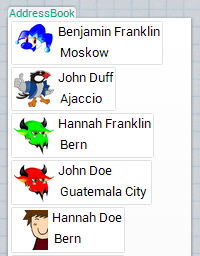
\includegraphics{img/AddressBook_whole.png}
	\caption[AddressBook visualization]{The representation of an AddressBook instance lists its contacts with few information.}
	\label{addressbook_whole}
\end{figure}

\begin{figure}[h]
	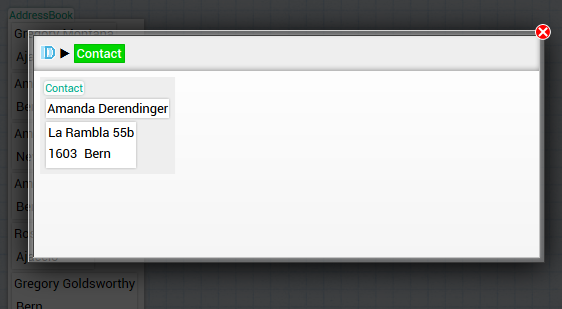
\includegraphics[width=\linewidth]{img/AddressBook_contact.png}
	\caption[Contact visualization]{When clicking on an element in the list, the selected contact is visualized with more detail and clickable inner objects.}
	\label{addressbook_contact}
\end{figure}

\nes{Describe breadcrumbs here. Including a reference to the word "bread crumbs". This should serve as a reference: http://www.amazon.com/Dont-Make-Me-Think-Usability/dp/0321344758}

In figure~\ref{addressbook_address}, our address object is on level 0 and its inner fields would render with more detail, but since they're only strings and numbers, no differentiation is made. \nes{Pick a better example, then. One where it does make a difference.} \meta{It does in figures \ref{addressbook_whole} and \ref{addressbook_contact}. There is always a point where you cannot get more detail, of course.}

\begin{figure}[h]
	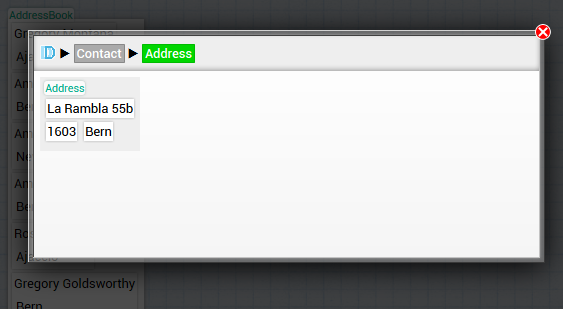
\includegraphics[width=\linewidth]{img/AddressBook_address.png}
	\caption[Address visualization]{Clicking on the address area inside contact opens a more detailed view of this \texttt{Address} object. Since its content only consists of \texttt{String} and primitive objects, there is no further detail revealed.}
	\label{addressbook_address}
\end{figure}

\nes{Really, honestly, there is no story if we can't make the point of being useful across time. That's how we claim to be better than debuggers. Without it, we have very little. Add an example of the same object being printed at different points in time.}

\section{Design}
Instead of immediately starting to implement, we followed several well-proven planning steps from literature to avoid costly redesigning or refactoring later on. The implementation followed Buxton's imperative to separate the design from the engineering processes\cite[pp.73--75]{Buxt07a}. Before writing a line of code, we designed the entire API and the resulting renderings on paper, involving numerous iterations of drawings.

\subsection{Sketching the Features}
In a previous paper, we had shown that textual output lacks features in cases of complex data structures, like matrices, that require accurate multidimensional arrangement for a good human perception, especially if they are nested. We also showed that custom textual object representations tend to exhibit a couple of frequently observable traits. Based on this information, we started to gather commonly used data types and sketch them to paper with a simple, meaningful appearance. Beside every sketched candidate rendering, we tried to think of a simple-as-possible but yet modular code snippet, that would imaginary render this image. Over time, while painting more and more candidates, we tried to converge our imaginary API, so we threw away outliers and repainted their object type in a more consistent way. When we had a consistent (still imaginary) API, we would take a step forward and consult third-party programmers for some feedback.
\nes{This entire subsection is useless. Show the sketches, show the code, be specific. This is just a poor summary of Buxt07a. Just reference Buxt07a, and explain what we did.} 

\subsection{Feedback For Hand-Made Sketches}
As soon as we had a consistent imaginary API and enough sample sketches, we stuck them to a wall and eventually asked other programmers to quickly look at those drawings and explain what they believe to see (figure~\ref{sketch-discussion}). If they immediately anticipated the virtual situation, it was a good example and we kept it. If most people failed to understand what a particular drawing meant, or even wrong conclusions were made out of it (figure~\ref{bad-sketch_left-right}), we either threw it away or tried to redesign, based on people's statements and then loop and ask them others about it. \nes{Too general to be useful. Examples, specifics. Which API was refined? What was the old version, what's the new?}
\todo{Loop back to the book.}

\begin{figure}[h]
	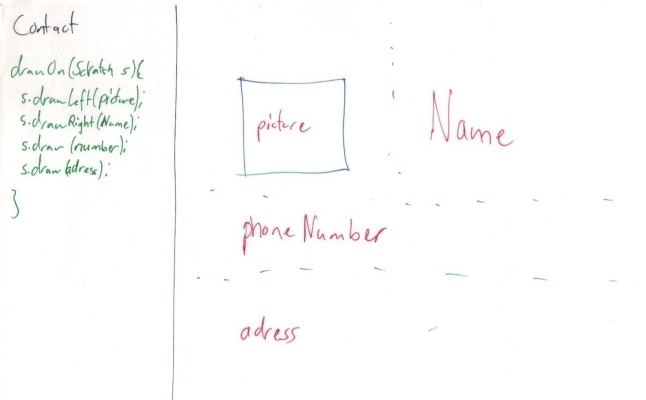
\includegraphics[width=\linewidth]{img/sketches/026.jpg}
	\caption[Bad sketch example: Left-right pattern]{One of the proposed types of API was traversing the canvas from top to bottom, divided into virtual lines. Users would be allowed to draw objects either on the left or the right part of its line, or just to take the line's full width. People mainly didn't understand the automatic creation of new lines. \texttt{drawLeft(object)} was mainly understood to take the left side of a bigger instance, e.g. the whole canvas.}
	\label{bad-sketch_left-right}
\end{figure}

\begin{figure}
	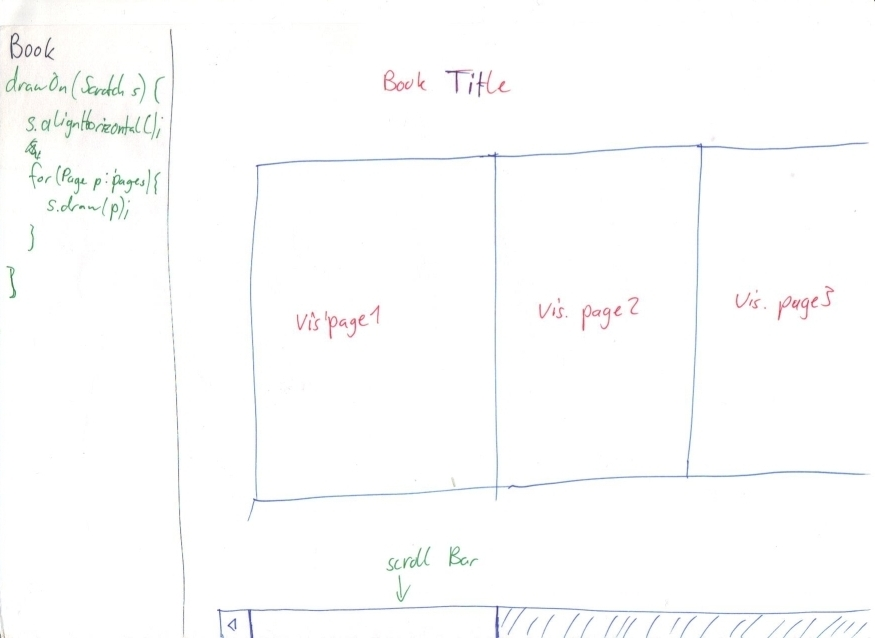
\includegraphics[width=\linewidth]{img/sketches/032.jpg}
	\caption[Bad sketch example: Horizontal and vertical alignment]{Another proposed API type was aligning all printed objects either horizontally or vertically, dependent on the user's choice. Though most asked programmers managed to quickly understand what the pattern on this sketch is, they immediately asked about further 2D structuring. One pointed out, that horizontal alignment would almost be equivalent to text printing, because it only supports one dimension.}
	\label{bad-sketch_align-h-v}
\end{figure}

\begin{figure}[h]
	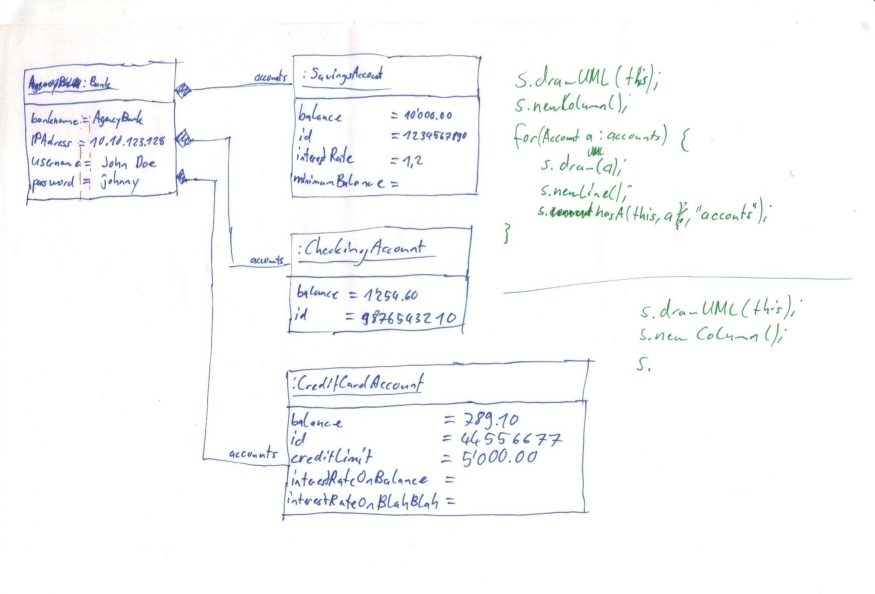
\includegraphics[width=\linewidth]{img/sketches/006.jpg}
	\caption[Bad sketch example: UML]{We considered using or at least supporting UML as an output format through the Doodleable interface. No one of the asked programmers supported this idea. The reasoning behind their refusal was that they had never actually used UML for any real project, since it would be too complicated for quick anticipation.}
	\label{bad-sketch_uml}
\end{figure}

\begin{figure}[h]
	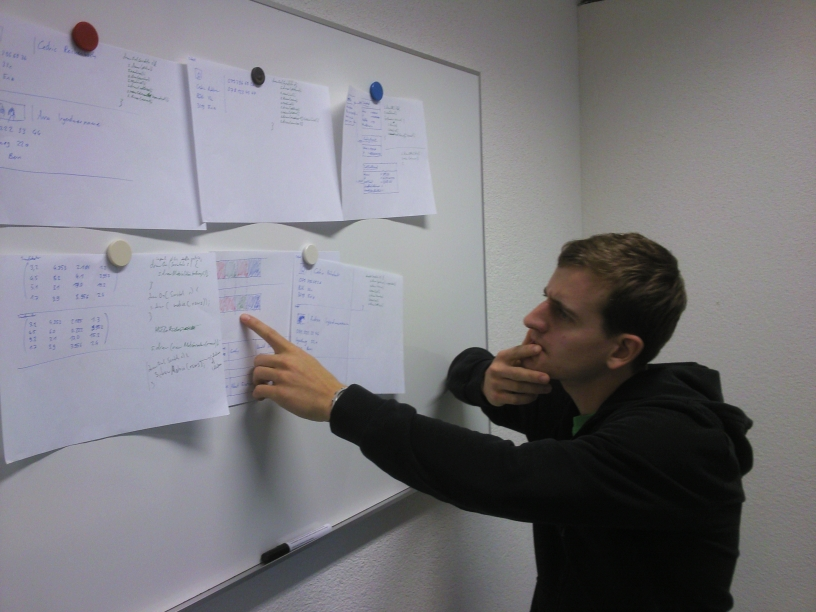
\includegraphics[width=\linewidth]{img/design-sketches_thinker.jpg}
	\caption[Confronting people with design sketches]{Programmers were confronted with our code snippets and corresponding design sketches, verbosely explaining their personal interpretation.}
	\label{sketch-discussion}
\end{figure}

\begin{figure}
	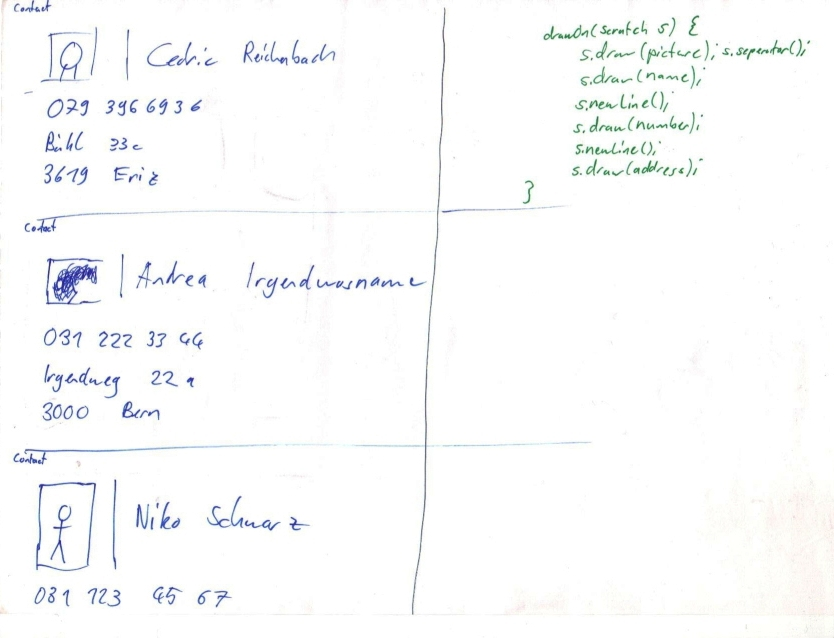
\includegraphics[width=\linewidth]{img/sketches/003.jpg}
	\caption[Good sketch: Cursor paradigm]{An API using the paradigm of a text cursor was adapted quickly by programmers. One asked question about this was why the second column would somehow float into the first one, since in common text blocks they're always separated. As a consequence, we adapted the traditional textbook pattern and strictly separate columns, which made the separator method obsolete as well.}
	\label{good-sketch_cursor}
\end{figure}

\subsection{Cursor Model for Canvas Painting}
For spacial navigation on a virtual canvas, a mechanism adapting the cursor paradigm of a simple text editor proved to be most intuitive for humans (figure~\ref{good-sketch_cursor}).
\nes{In conflict with the "nutshell" section. Move contents up, or delete.} Initially, the virtual cursor is placed on top left of a virtual canvas. Printed objects are aligned side by side like words in a text until the user creates a new line and the virtual cursor jumps back to the left, vertically shifted of course. After a couple of lines, a user may want to continue their painting beside of the already printed parts instead of constantly appending content to the bottom. For this, they can create a new column, which is attaches to the right side of previous one (figure~\ref{canvas-illustration}).

We attribute the supremacy of this method to the principle of standardization\cite[pp. 200--203]{Norm88a}. This means that similar usage patterns make life easier for users, since they only need to learn it once and then apply everywhere. Virtually traversing an area from top-left to bottom-right, separated in lines and eventually in columns, is the way how text is written in western languages. Especially programmers, who use text editors on a daily basis, can therefore quickly adapt and apply this principle. Other technologies have adopted this paradigm as well: \verb-System.out.println()- uses a cursor position and text flow, divided into lines. Java's AWT package uses canvas coordinates that originate on the top-left corner.

\subsection{Smart Behaviour versus Configuration Hell}
When designing user interfaces, one basic decision must be taken: How much configuration options should it contain? Either a lot of settings are left to the user let them take part on the design process. Or the default design is made to fit everyone as good as possible. We decided not to treat everyone as designer
\cite[pp95ff]{Buxt07a}
\cite[p155]{Norm88a}
but take away design decisions from them by creating sophisticated defaults.
As a result, there is no settings dialogue or file for DoodleDebug. \nes{Nice!}
\subsubsection{Smart Scrolling}
DoodleDebug implements the scrolling behavior of MUSHClient\footnote{\url{http://www.gammon.com.au/mushclient/}} and mIRC\footnote{\url{http://www.mirc.com}}. That is, when the most recent doodles are currently in view and a new doodle appears, the view port will scroll to keep the newest doodles in view. If, however, the view port is not showing the most recent doodles and a new doodle appears, no scrolling occurs. 
This is probably in line with the user's intent. If they're looking at the most recent doodles, they probably are tracking the most recent doodles. If, however, the most recent doodles are not in view, they're studying a specific old doodle that should remain in view. 
This took some engineering effort, since HTML provides no built-in support for scrolling on content growth.

\subsubsection{Focus When Likely Desired}
When a new Doodle occurs, DoodleDebug chooses whether or not to notify the user. 
DoodleDebug operationalizes the time since the last doodling to estimate if the developer benefits from being notified by a recent doodle. Thus, frequent doodling does not trigger notifications, and the developer is not continually interrupted. \nes{What is the threshold? \meta{4 seconds.} How established? \meta{Empirically. Since we didn't have too much data from the study, it's still pretty arbitrary.}}
The problem of unwanted focus change has been observed in our study. A candidate manually disabled the console's focus gathering because they were working in another view and it constantly jumped back (see \ref{console-focus-problem}).

\section{Implementation}
\nes{Niko: The intro paragraph needs a complete re-write. I will probably do it once I've read the rest of the section.}
The efforts made in analyzing classical debugging tools and how programmers behave when interacting with them all aimed on implementing a tool which would actually fill the mentioned problematic gaps. Though the implementation part is not the main theme of this paper, we will point out a couple of general conceptual patterns as well as relevant technical aspects in this section; further descriptions can be found in the appendix.

\subsection{Rendering algorithm}
If the user clicks on a doodle, DoodleDebug \emph{Semantically Zooms}\cite{Wood98a} into the doodle he clicked on.
Object visualizations are divided into levels of nesting, where level 0 represents outermost objects, referenced in \verb-Doo.dle(object)-, level 1 objects are (semantically) nested ones inside level 0 \emph{etc.} Saving space is achieved by only completely rendering level 0 and 1 objects, and use a smaller representation for objects of level 2. Level 1 objects are clickable, which will cause them to be repainted as new virtual level 0 objects, so previous level 2 objects will move to level 1. This pattern allows to arbitrarily explore an objects nesting tree, similar to a debugger.
\nes{Separate this better from the "nutshell" section. Here, focus on the levels and their consequences. Move the explanation of how it works to the nutshell section. Here, only explain the "how".}

\subsection{User API}
DoodleDebug's public API can be divided into three parts:
\begin{enumerate}
\item The \verb-Doo.dle#(Object)- method, which is a drop-in replacement for \verb-System.out.printLine#(Object)-
\item The \verb.Doodleable. interface, which can be implemented by users to define two methods for simple and quick custom object representations
\item \verb.RenderingPlugin.s as plugins for DoodleDebug, which give fine-grained control over the html and css output for a class without having to modify it. \nes{Hmm.}
\end{enumerate}

\subsubsection{The Doodleable Interface}
In our previous paper, we had proposed a pattern where objects should contain information about how to represent them. \nes{Enough with those generalities!} During the planning phase, we continuously improved \nes{You keep asserting that. Don't. Just show it, by showing sketches and details.} a initially rough prototype of such an API until it converged to a form that met our requirements of intuitiveness and simplicity. For adding rendering information to an object, its class must implement the \verb.Doodleable. interface. \verb.Doodleable. contains two methods, \verb.doodleOn(DoodleCanvas c). and \verb.SummarizeOn(DoodleCanvas c). in order to support semantic zoom by having two representations with different levels of detail. The pattern behind the \verb.DoodleCanvas. is a virtual canvas with a virtual cursor behaving similarly as those in common text editors.

\subsubsection{Providing Plugins to DoodleDebug}
The html and css output is generated by plugins, inheriting from \verb.AbstractPlugin..
The default visualizations that DoodleDebug ships are all implemented as Plugins.
\nes{Describe the plugin selection mechanism.}

\paragraph{Rendering the Output}
For displaying and handling HTML code and related web technologies, Eclipse provides the package \verb-org.eclipse.swt.browser-, which among others includes the \verb.Browser. class to render and integrate into the Eclipse UI. This \verb.Browser. class is not completely platform independent. It uses the default \nes{What does "default" mean here?} browser rendering engine of its current host operating system. When running on Windows for instance, Internet Explorer's rendering engine is used, even though Firefox is set as the System's standard browser. This fact forced us to be even more careful with the usage of HTML5 features, because their support varies between Browsers.

\subsection{Communication between Java Virtual Machines}
DoodleDebug renders its output into a view \nes{What's a view tab?} (``window'') \meta{Those are just the view parts in eclipse, called ``views''. E.g. an editor is a view. The project explorer is a view. The console is a view.} inside eclipse, so we implemented it to have the main part running in the same VM as eclipse for convenience. Since runtime information about objects and rendering calls must be provided from the user's VM to the eclipse VM, a solid communication mechanism is needed. We use SIMON (Simple Invocation of Methods Over Network)\footnote{\url{http://dev.root1.de/projects/simon}}, a library for object-oriented remote communication in Java. It allows to create a registry on a specified port of localhost and add a Server object to it. Clients can find the server through this registry and send messages to it by calling it's methods with simple objects like Strings as arguments.
\nes{This is hard for me to fix before we have a good section on across time debugging to motivate why we keep old versions around. Please urgently write that.}

\subsection{Providing Code from Eclipse Plugin to Workspace}
\meta{Appendix?}
As DoodleDebug works by calling its methods directly from user programs, some code needs to be exposed to the scope of a user's program. On the one hand, all API methods must be visible from user projects. On the other hand, users should only see a minimal amount of DoodleDebug's code in order to prevent them from using it in an unintended way and cause bad behavior. The compromise made between those two requirements was to mainly provide simple, well-documented interfaces (such as \verb-Doodleable- and only show a proxy of fully implemented classes (e.g. \verb-Doo-).
\nes{Delete and re-write by doing the following. Explain clearly the end-user process of using DoodleDebug. Answer clearly: If a user chooses to use DoodleDebug, will he have to include DoodleDebug into his production code? (yes.) How much of it? (Not much.) What happens if a coworker doesn't have the plugin installed (It'll break, but we're working on chickening out and printing to System.out.println in that case.)}

\subsection{Serialization for the Transport between VMs}
SIMON only allows transporting simple data types such as Strings, so every object is serialized before its transportation. For this purpose, we make use of XStream\footnote{\url{http://xstream.codehaus.org}}, a simple serializing library, originally created to serialize Java objects to XML and back again. Because of it's modularity, it also allows to serialize to JSON and comes with a built-in mapping for this. Because of XML's more verbose syntax and therefore bigger space/time consumption in many cases, we decided to use JSON as first choice, with a fallback to XML if errors occur. This is necessary because standard JSON cannot handle circular references, it lacks the ability to append attributes to entities and therefore cannot index them in order to reference to a parent id in case of a circular reference. Obviously, there are workarounds for this issue, but the fallback to XML does not take as much time that users could even recognize it is happening.
\nes{Meh. Explain that it would be nice to only transfer needed parts of the object graph, but that we don't have that currently. XStream is an out-of-the-box solution with severe limitations, memory-wise. Explain (later?) that this should be tackled by a mixture of more efficient storage and limiting the object database in size, like an LRU cache.}

\subsection{Communication between Java and JavaScript}
\subsubsection{From Java to JavaScript}
DoodleDebug renders its output into a dedicated tab inside the Eclipse UI, using Eclipse's \verb.Browser. class. To append newly rendered objects to the output screen, a naive approach would be to just cache the current code on Java side and in the case of freshly added object renderings, just repaint the whole html page. 
This has some disadvantages: A refreshed page may always jump back to the top, and even if it does not or it is avoided by jumping back down with JavaScript, it would flicker anyway for the split of a second. 
Instead, we use \verb.Browser.'s \verb.execute#(String script). method to sneak to-be-added html into the browser. The html to be added is wrapped into JSON and then passed into the browser. Inside the browser instance, our own \verb.addCode(code). method adds a new doodle \nes{Why on earth is called addCode if it adds doodles?!} to the output. The rendered html of the doodle also contains an identifier to the object in the object database, so that later clicks will allow semantic zoom, as discussed earlier\nes{Add reference}. 
\nes{The object store is not discussed properly at all. Neither is the connection between JS and the object store.}

\subsubsection{From JavaScript to Java}
\nes{I don't understand this. Don't name the parts of our solution by language. Here are the components: inside the browser, inside the Eclipse plugin, inside user code, and there is the object database. How are they connected?}
\meta{Might be partially irrelephant $^\circ$j$^\circ$m}
Every rendering of Java objects to html is done in Java, so the output entity can only operate as a thin client.
In order to make output interoperable, communication from JavaScript to Java is necessary, e.g. if an object is inspected and it's nested objects are not yet rendered. Because the output is rendered as html into a Browser, it is of course encapsulated from it's environment, which is a good thing for general portability of web site, but in this special case, it was a drawback. There is no such thing like a JavaScript-Method like "\verb.sendToBrowser(message).", so we had to find some workaround to notify the Java instance about occurring events (e.g. lightbox closing) on one hand and be able to provide some arguments (e.g. which object to render) on the other hand. Using AJAX calls on localhost would probably cause some tedious delays, break encapsulation and just be bad style.

The solution we finally came up with causes no remarkable delays and stays inside its dedicated context: Eclipse's \verb.Browser. class allows to append event listeners for the case that its \verb-window.location- is about to change. We defined a pseudo-protocol \verb-doodledebug- and append some message to it, maintaining syntax limitation such as no white space. On Java side, a listener handles all location change events; if an event's target location fits the pseudo-protocol's pattern, its "message" is parsed and desired steps executed. The location change itself is cancelled, so the user stays on the same page. For instance, if an object is clicked and should be inspected inside a lightbox, this item's id is determined and the window location set to \verb-doodledebug:<id>-. On Java side, the object to render is determined from this id, rendered and a message with html code sent back to JavaScript again.


\section{Study}
\nes{On how to write up a user study like this, see "http://research.microsoft.com/en-us/um/redmond/groups/hip/papers/ko2007bugfixing.pdf"}

The concept of DoodleDebug is especially based on studies about human interaction with classical debugging tools. \nes{I'm sure that Ko did not start his user study with the word "essentially"} 
Therefore, a study comparing interaction with classical tools to selfsame with DoodleDebug under similar conditions promises information about the actual improvement of DoodleDebug in relation to classical tools. The study should focus on problems considered to occur frequently in similar forms as well as special cases, where the choice of debugging tools may be more crucial than in others.

We chose the form of a qualitative rather than and quantitative study. This appeared as a more reasonable choice due to limited candidate resources and our goal of finding causalities rather than just proving a previously made statement. For a qualitative study, we would have not only have needed a number of candidates big enough for statistically relevant data, but also have strictly defined environmental conditions to assure consistency. Also, less semantic insight into the candidate's debugging behaviour could have been gathered\cite[pp. 13--15]{Lang09b}.

\subsection{Study Session Setup}
A fully functional version of DoodleDebug was used, most probably the equivalent to a "release candidate". It was run inside Eclipse 4.2 (Classic edition), using a ThinkPad T410 with Windows 7 (x64) and an additional mouse (2 buttons + wheel, standard size). The screen was captured during the whole session and one instructor sitting beside the test subject for problem explanation and protocol. Before the actual testing, the user had 15 - 30 minutes to work through a tutorial and play around with DoodleDebug inside a sandbox. At this time, the instructor was allowed to answer questions and support the subject.\\
For the actual session, there were 3 different small programs containing some manually inserted bug, which they had to find and eliminate. For one or two of them, they were allowed to use DoodleDebug and for the other one or two respectively, they had to fall back to classical tools. The permission to use DoodleDebug on a particular problem changed with every study session, i.e. if subject 1 was allowed to use DoodleDebug on problem A, then subject 2 would not be allowed, but subject 3 would. The reason for letting some candidates only use classical debugging tools was to have a reference of behaviour in order to show that they are not trivial and detect what particular sub-problems they pose in detail, so we would see if DoodleDebug enables better approaches to solve them. Obviously we could not let people solve the same problem in both modes, or they would have been prejudiced by the solution they found before.\\
A subject was always working on a problem until it was completely solved, none of them needed more than 30 minutes for all problems together.

\subsection{Posed Problems}
\paragraph{Sorting}
A couple of grey scale \verb.Color. objects are put into a \verb.List. and then sorted using a custom \verb.ColorComparator., which should sort by brightness. The result then is compared to a hand-built \verb.List. which initially has the expected order. This test fails and it's the subject's task to find out what is ordered wrong, i.e. if there is a clear pattern, and to fix this bug. Subjects have access to all of the source code and are allowed to manipulate it.\\
Solution: In the comparator, completely black colors are wrongly treated as complete white.

\paragraph{Serialization}
Phone book contacts are modeled using \verb.Contact. and \verb.Address. objects. They should be serialized using a \verb.SerializingUtil. (simulated serialization only) and de-serialized afterwards.
Those mechanisms are executed with example data, but comparison of a contact object before and after serialization fails. The subject's task here is to find out what parts of the contact object were broken and why, i.e. fix the bug. Subjects have access to all of the source code and are allowed to manipulate it.\\
Solution: In the \verb.SerializingUtil., every field of type \verb.long. is casted into an \verb.integer. before serialization and back into a \verb.long. afterwards. This causes a field called \verb.phoneNumber. of \verb.Address. to be changed into some negative value.

\paragraph{Decimal Alignment}
A class \verb.DatabaseUtil. is a black box simulating access to an imaginary database by returning a two-dimensional array of \verb.float. when calling it's only method \verb.getData().. Subject know that in the returned table, there are duplicated tuples and have to name them. Because they have no access to source code, they need to rely on received data only and also cannot fix the bug.\\
Solution: There are two pairs of fitting rows (3 \& 8, 6 \& 9).

\subsection{Candidates}
To respect privacy, the real names of our test subjects have been replaced by character names of the usual Radio Spelling Alphabet, enumerated in order of their participation.

\subsubsection{Education and Experience of Each Candidate}
\paragraph{Alpha} % Oskar Truffer
\begin{enumerate}[$-$]
\item B.Sc. in Mathematics, Minor Computer Science 60 ECTS
\item Master Student in Computer Science
\end{enumerate}

\paragraph{Bravo} % Remo Diethelm
\begin{enumerate}[$-$]
\item B.Sc. in Computer Science
\item Master Student  in Computer Science
\end{enumerate}

\paragraph{Charlie} % Andrei Chis
\begin{enumerate}[$-$]
\item M.Sc. in Computer Science
\item Ph.D. Student in Computer Science
\end{enumerate}

\paragraph{Delta} % Julian Schelker
\begin{enumerate}[$-$]
\item B.Sc. in Computer Science
\item Master Student  in Computer Science
\end{enumerate}

\paragraph{Echo} % Raffael Krebs
\begin{enumerate}[$-$]
\item M.Sc. in Computer Science
\item Working as Software Engineer, 1 year of experience
\item Minor experience in Eclipse plugin development (master thesis)
\end{enumerate}

\paragraph{Foxtrot} % Roger Kohler
\begin{enumerate}[$-$]
\item B.Sc. in Computer Science
\item Master Student  in Computer Science
\end{enumerate}

\paragraph{Golf} % Ueli Scheidegger
\begin{enumerate}[$-$]
\item Lic.rer.pol. in Economics, Minor Computer Science 60 ECTS
\item Working as Software Engineer, 15 years of experience
\end{enumerate}

\subsubsection{Different Problem Approaches}
Depending on study session with our candidates, we could observe different patterns of approaching a problem with classical tools.
\paragraph{System.out.println()}
5 out of 7 subjects (all except Delta and Echo) made use of this mechanism to visualize runtime data. It's quick and Alpha for example argued with laziness to open a debugger or to stare at foreign code. Also, they can compare things, either two different objects as posed in the sorting problem or the same object at different points in time, as in the Serialization problem. Both is not directly possible with a classical debugger like the one coming built-in with Eclipse classic.
\paragraph{Debugger}
Four subjects (Bravo, Delta, Echo and Foxtrott) used the eclipse debugger to inspect objects, only Delta and Echo used it exclusively. The argumentation for this usage was that debuggers are more powerful in comparison to System.out.println(), because they allow to inspect objects dynamically and additionally provide simple improvements of standard textual representations (e.g. arrays are represented in the form of \verb-[objectA, objectB, ...]- instead of \verb-[Ljava.lang.Object;@4cb162d5-. But Echo also missed the feature to compare two objects, even at the same point in time they could not manage to do so.
\paragraph{Source Code Staring}
As mentioned before, debugging tools were mainly developed to avoid the need of staring at code, and most people found this the most annoying part, especially because it was code they had not written on their own. Nevertheless, subject Golf solved the Serialization almost only by using this method. They tried to comprehend the logic of the problem's \verb.SerializingUtil. and thus, in contrast to others, found the problem source at the same time as the semantic problem itself. To be exact, they located where the problem was (long casted to int) and used System.out.println() only to check what it resulted in.

\subsubsection{General Problems}
\paragraph{Console Keeps Stealing Focus}
\label{console-focus-problem}
When some output is printed onto the console, it gains the UI's focus by default. Due to the problem setup, every program initially used to throw an exception at the end of it's execution, signaling the problem has not been solved yet. Every user experienced the following problem at least once: They were using DoodleDebug and therefore had this view tab opened when the exception was thrown and eclipse switched to the console. Only Echo managed to disable its focus-on-change setting, the other subjects just switched back to the DoodleDebug view tab after a few seconds.

\subsubsection{System.out.println()}
\paragraph{Homogenous Output}
Purely textual output is poor in terms of formatting and therefore makes it harder for users to classify different parts as they always look similar in terms of size, color and alignment. When solving the sorting problem, subjects were slowed down due to this fact. Beta for instance firstly iterated over the wrongly sorted color list to print each element and then stared at the (unaligned) numerical values of red, green and blue color components. After they had found out that a black element was at the end instead of the beginning, they could go on searching what had caused the problem. Subjects using DoodleDebug already had built-in renderings for \verb.Collection. and \verb.Color., which enabled them to visualize it by only using one call. Charlie Doodled the wrongly sorted color list and the correct one that was used as ground truth for comparison. They instantly noticed their similarity and pointed out that black is on the wrong side of the list.

\paragraph{Uninspectable and Useless Output}
The standard implementation of \verb-System.out.println()- prints class name and object hash for non-primitive objects. Output printed to a console is static and can not be inspected. If an object's representation lacks a particular piece of information, the programmer will need to go back into the code and either change the \verb.toString(). method of its class or manually gather information from outside and print it. In our study, Charlie was the only subject to override \verb.toString(). methods after firstly using their standard representation. They implemented it by printing out all fields of an object: \verb.Contact. was represented by\\
\verb-"name: " + name + ", address: " + address-,\\
whereat \verb.Address. was represented by\\
\verb-"street: " + street + ", phoneNumber: " + phoneNumber + ", city: " + city-.
This representation recursively breaks down a \verb.Contact. object into primitive types, which can be easily represented by text. Alpha produced a very similar output, but instead of overriding \verb.toString()., they extracted all fields from outside using getter methods directly inside the System.out.println() method. Golf only used System.out.println() as help for code inspection, they printed one particular primitive field at a time without considering its containing object.\\
Another approach to solve insufficient output was to switch from System.out.println() to the debugger, observed on Bravo and Foxtrot.\\
DoodleDebug includes an objects fields in it's standard rendering (if there are not too many) while still labelling its class name. All 3 subjects (Bravo, Delta, Foxtrot) using DoodleDebug for the serialization problem managed to find the changed field instantly after calling \verb-Doo.dle()- once before and once after the de-/serialization step.


\subsubsection{Debugger}
\paragraph{Comparison Between Objects}
The built-in eclipse debugger only allows to inspect one object at one point in time. As the serialization problem consists of two objects unexpectedly  being unequal, part of the debugging process was somehow comparing them in order to find their difference. Every subject except Golf did this, Golf only tried to understand the serialization and de-serialization process to find out, where the implementation has mistakes. Echo never used \verb-System.out.println()- so they also attempted to compare objects before and after serialization using the debugger. Even though the debugger supported simple and fast inspection to any point inside the object, Echo explicitly pointed out that they miss the feature to inspect two objects simultaneously instead of memorizing small pieces and going to the other one for comparison.

\paragraph{Non-Selective Output}
Eclipse's Java debugger simply lists all contents of an object, since there is no information about relevance of its respective parts. In particular, interfaces may specify a imaginary concept and be used in in the declaration context for better overview, but for creation of an instance, a full class implementing this interface is needed. The debugger is working at runtime and therefore only knows the instantiated type of an object, so it will visualize all properties and contents of this, potentially resulting in a overly verbose output. We observed this on the color list problem, where \verb.ArrayList. was used as implementation for the interface \verb.List.. Subject Bravo initially tried to perceive the structure of a list right after sorting by pausing the program  using the debugger and inspecting the mentioned list (figure ~\ref{debugger_color-list}), but instantly gave up and switched to writing a \verb.for. loop which sequentially prints out all elements using \verb-System.out.println()-. If the standard output of DoodlDebug does not fit a users needs, it can be adjusted through of the two described methods, the simpler Doodleable interface was used in this context by Alpha. \todo{Screenshot of Doodleable usage}
\begin{figure}[h]
	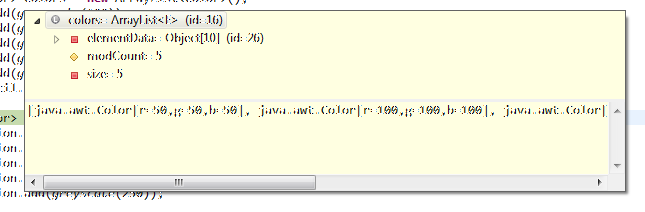
\includegraphics[width=\linewidth]{img/debugger_color-list_remo.png}
	\caption[\nes{Screenshot unreadable.} Bravo using the debugger for a color list]{Eclipse's debugger visualizes all fields of an object's runtime type (ArrayList)}
	\label{debugger_color-list}
\end{figure}

\todo{Are there more examples? (Good ones)}
CodeBubbles's\cite{Brag10a} debugger allows users to open bubbles by hand that represent states in the debugger. Thus, many old states can be on-screen. However, all old state is triggered thru direct user interaction. Unlike System.out.println, or DoodleDebug, where all printing happens from the program.

\todo{What further related work is worth mentioning?}
\nes{This gaming guy that would overlay time frames in his output.} \meta{What? Who?}

Finding the source of problems in program code is an omnipresent issue in computer science and therefore a recurrent research theme. Previous studies about human behavior when developing and especially debugging code were good hints to point where DoodleDebug should be going. We filtered relevant data out of them and aligned them with our research efforts, resulting in a separate paper.


\section{Related Work}
\todo{text}

\subsection{Previous Paper}
In a previous paper\cite{Schw11b}, we analyzed generally used patterns for textual representation of open source projects and showed basic conceptual issues preventing useful representations of certain data types. Following that, we outlined a concept automatically including information mostly used in custom textual representations and supporting ``difficult'' data types that prevent powerful renderings in textual form.

\subsubsection{Mining SqueakSource}
We had programmed a simple Smalltalk data miner, which fetched all projects from SqueakSource, searched all classes overriding Smalltalk's \verb.printOn:. method, which is roughly equivalent to Java's \verb.toString(). in its meaning to programmers; namely it provides a textual representation of an object in order to print it to a console. In a next step, we manually went through the received \verb.printOn:. code snippets (590) and searched for repeating patterns.
\begin{itemize}
	\item 44 used ASCII graphics to build two-dimensional structures.
	\item 137 wrapped their printed instance variables using parentheses.
	\item 219 called \verb.printOn:. of their super class.
	\item 452 included their class name.
\end{itemize}
For DoodleDebug, we tried to consider those patterns and include them as well as possible and eventually include them in every output without the need of user manipulation. If not, they should be easily produced through an API.

\subsubsection{Text is not always powerful enough}
In the same paper, we argued that there are data structures\del{,} where using classical console printing contains clear disadvantages, demonstrated using Arrays of two-dimensional matrices as an example of multi-dimensional structures. Objects with independent textual representation methods can only be listed vertically, which does not allow nesting with a consistent and thus clear layout (figure~\ref{nested-matrix-problem}). This nesting problem could be solved, if representation methods would not be restricted to one-dimensional text only (figure~\ref{nested-matrix-idea}).
\nes{You're repeating the old paper, and I don't see why. Use it where necessary. It isn't at all necessary here.}

But simple textual output has even more restrictions than just the one caused by its single dimension: Colors are not supported in general, printing images is impossible and already printed line cannot be deleted, which limits formatting as well as the lack of free spacial positioning.
\nes{Move to the discussion of System.out.println. It is one of its shortcomings. Has nothing to do with our old paper. But do attribute it to our previous work.}

\begin{figure}[h]
	\begin{verbatim}
    an Array()

    an Array(
    MatrixTransform2x3(
        2.0 0.0 0.0
        0.0 2.0 0.0
    ))

    an Array(
    MatrixTransform2x3(
        2.0 0.0 0.0
        0.0 2.0 0.0
    ) MatrixTransform2x3(
        0.707107 -0.707107 0.0
        0.707107 0.707107 0.0
    ))
	\end{verbatim}
	\caption[Bad nesting of 2D-matrix array]{Textual visualization of an array of 2D-matrices in Smalltalk}
	\label{nested-matrix-problem}
\end{figure}

\nes{I don't think we can keep nested-matrix-idea. This is a paper about the really-existing DoodleDebug. If we don't have a rendering, we don't have it. Don't mention it.}
\meta{But we have a special rendering for matrices/tables: Rectangular 2D-Arrays and 2D-Collections are rendered specially. If they contain numbers only, those get aligned by decimal point.}

\begin{figure}[h]
\raggedright
	$\{\}$
	\begin{verbatim}
	
	\end{verbatim}
	$\{\begin{pmatrix}
	2. & 0. & 0. \\
	0. & 2. & 0. \\
	0. & 0. & 2.
	\end{pmatrix}\}$
	\begin{verbatim}
	
	\end{verbatim}
	$\{\begin{pmatrix}
	2. & 0. & 0. \\
	0. & 2. & 0. \\
	0. & 0. & 2.
	\end{pmatrix},
	\begin{pmatrix}
	0.707107 & -0.707107 & 0. \\
	0.707107 & 0.707107 & 0. \\
	0. & 0. & 1.
	\end{pmatrix}\}$
	\caption[Ideal nesting of 2D-matrix array]{Possible visualization of an array of 2D-matrices without the restriction to 1D-text}
	\label{nested-matrix-idea}
\end{figure}

\subsection{Whyline for Java}
Whyline\cite{Ko04a} is a Java library that should answer why and why not questions about a program's behavior. Developers  click on a piece of either graphical or textual output and ask questions about the cause of its properties. Whyline then tracks back the program execution to the line of code where this particular field has been changed for the last time and visually reports it to the user, including the causal chain leading to it. Whyline aims on connecting properties of output to code snippets. In other words, it answers the "why" question. DoodleDebug visualizes objects and helps to understand what properties objects have and how they evolve over time. It answers the "what" question. By now, Whyline only supports output on \verb-java.awt.Graphics- and \verb-java.io.PrintStream- objects and is developed with closed source only, but from a conceptual point of view, those two technologies could be combined and eventually enhance each other.

Compass\cite{Lien09a} offers the user to trace objects back in time. Whereas DoodleDebug keeps the old states of objects that were doodled, Compass keeps a database of expired stack frames. While Compass must pre-emptively store stack frames that may or may not be relevant, DoodleDebug only keeps snapshots that the developer specifically marked as interesting.

\section{Future Work}
\nes{This is out of hand. We may or may not keep the "split doodleable interface" thing. Though I still think that should just be fixed and listed as an accomplishment, not as future work. The rest of this section should go.} \meta{We cannot easily split it, because it would generally break the paradigm of complete semantic zoom, i.e. we would need case distinction and fallback. Also: Change the API, test everything, re-write tutorials and examples etc. This cannot be safely done in 2 days, just estimating from the last time we changed the API...}
Besides proving things right, our study revealed some problems as well. As they only show that a problem exists but don't provide exact information about its cause, further research might invest in analysing them and propose accurate solutions.

\subsection{API}
\todo{Text}

\subsubsection{Split The Doodleable Interface}
\paragraph{Problem}
As already described, the \verb.Doodleable. interface contains two methods for object representation, one for a detailed and another one for a summarized variant. This structure greatly allows integration of semantic zoom because it forces user-provided information about content importance. However, study subjects eventually were unsure about the semantic meaning of those methods. Echo, for instance, verbally communicated his confusion about their difference; after going back to the documentation, everything was clear. Alpha did not show any special reaction when implementing the Doodleable interface for the first time, but simply "delegated" the zoom mechanism by replacing \verb-c.draw(object)- from their \verb.doodleOn(Canvas c). by \verb-c.drawSmall(object)- in their \verb.doodleSimplifiedOn(Canvas c)..

\nes{Why is this future work?! Just solve it, no?}
\meta{It's not proven. Would this REALLY be better?}
\nes{Sure it's proven. Just read your study. Not a person in your study implemented the interface that the study was trying to examine.} \meta{Just because this is isn't good doesn't mean the other is better. If we split it, we can throw away semantic zoom, as no one will ever implement SmallDoodleable if they don't have to (I'd even make a bet...).}

\paragraph{Possible Solution}
An approach for resolving this issue would be to split \verb.Doodleable. into two interfaces containing one single method each, let's say \verb.Doodleable. and \verb.SmallDoodleable.. For support of semantic zoom, users could simply implement both interfaces; if not, they would likely only use the standard version method. People implementing both interfaces would possibly make sure to first inform themselves of the respective semantic meanings and not run into previously mentioned slips. A user study comparing two groups, one using a single interface like before and another one using  the proposed setup, could help to determine if it's an actual improvement. Anyhow, this solution would introduce new conceptual problems: What should happen if a user only implements \verb.SmallDoodleable.? Should DoodleDebug try to guess a way for semantic zoom of objects only implementing one interface or just ignore it and always use the same method for rendering?

\subsubsection{Include Variable Name in Visualization}

\paragraph{Problem} When people are debugging parts of their code and use object visualizations, it is obviously essential for them to map a visualized element to its corresponding object in code for simple use cases, the object's class name is already good hint and widely used for custom textual representations as well\cite{Schw11b}, but it may become unclear if one is working with many different instances of the same class. Echo, who was only using the debugger beside DoodleDebug, stated it would be practical to see which object has which name in order to directly associate them with code snippets.

\paragraph{Possible Solution}
The very first step in this issue should be to clarify if it's technically possible to gather information about variable names during runtime. If so, the next question would be which context is relevant, since objects can be referenced to through different names from different contexts; probably the context where \verb-Doo.dle(object)- was called would be the only reasonable choice. For objects with no names in this context, e.g. inline objects, a meaningful replacement would need to be found to avoid user confusion. A good solution for UI integration might be achieved by pen and paper work; draw some sketches, show it to programmers and ask about their intuition.

\subsubsection{Link Visualization to Source Code}
\paragraph{Problem}
Mapping a visualized entity to its triggering line (\verb-System.out.prinln(object)- or \verb-Doo.dle(object)-) in code is not a problem if this line has just been written. It might become one if either if it has been written a long time ago or by another programmer, such that the current user does not know where the call is originating. Class name and content of an object may not always be helpful to find it, so full text search must be used to find the right code sequence. This can be costly as well if there is a big amount of code and/or a big amount of other calls for object visualization. As the projects in our study were only small and used one per user, we couldn't prove the mentioned problem as a fact, so a small study or survey could reveal how prevalent it actually is.

\paragraph{Possible Solution}
By utilizing Java's stack trace, the call origin could be determined and integrated in the rendering. As it is an Eclipse plugin, some mechanism could be created to directly create a clickable link to the corresponding source code line of a visualized object, similarly to the mechanism used for printed stack traces of Throwables. A good UI integration could again be achieved with pen and paper interviews.

\subsubsection{Simultaneous Usage of Multiple Eclipse Instances}
\paragraph{Problem}
The communication between DoodleDebug's client (API) and server (plugin) side happens through a Socket on a special port of localhost without any further identification between the two. The main problem when trying to achieve a correct mapping between running client and server instances is that clients have no safe way of gathering information about the Eclipse instance they're running inside. This is of course intended by IDE developers, as the running program should be completely independent, so working solutions might break in special cases or future IDE versions.
\paragraph{Possible Solution}
If the client side has no ability to autonomously get information about the Eclipse instance, it has to be provided from outside. One way would be to put a file containing a unique identifier of the running eclipse instance into the client's classpath from server side. One disadvantage of this solution is that it won't work when multiple instances try to run the same program.

\section{Conclusion}

\meta{What is the focus of this section? How big should it be? Just a paragraph of summarizing the results or (much) more detail? Personal opinions strictly prohibited?}
\nes{Conclusions are the facts that remain when all is said and done. They're the outcomes of the study, the things that last. They're the answers to the questions asked in the introduction. The section should be short.}

\section{Appendix}
\meta{Do we write an introduction to appendix as well?}

\subsection{Download}
The DoodleDebug Eclipse plugin and additional documents can be downloaded from \url{http://scg.unibe.ch/wiki/projects/DoodleDebug}.

\bibliographystyle{plain}
\bibliography{bib/scg}

\end{document}
